% Options for packages loaded elsewhere
\PassOptionsToPackage{unicode}{hyperref}
\PassOptionsToPackage{hyphens}{url}
%
\documentclass[
]{book}
\usepackage{amsmath,amssymb}
\usepackage{lmodern}
\usepackage{iftex}
\ifPDFTeX
  \usepackage[T1]{fontenc}
  \usepackage[utf8]{inputenc}
  \usepackage{textcomp} % provide euro and other symbols
\else % if luatex or xetex
  \usepackage{unicode-math}
  \defaultfontfeatures{Scale=MatchLowercase}
  \defaultfontfeatures[\rmfamily]{Ligatures=TeX,Scale=1}
\fi
% Use upquote if available, for straight quotes in verbatim environments
\IfFileExists{upquote.sty}{\usepackage{upquote}}{}
\IfFileExists{microtype.sty}{% use microtype if available
  \usepackage[]{microtype}
  \UseMicrotypeSet[protrusion]{basicmath} % disable protrusion for tt fonts
}{}
\makeatletter
\@ifundefined{KOMAClassName}{% if non-KOMA class
  \IfFileExists{parskip.sty}{%
    \usepackage{parskip}
  }{% else
    \setlength{\parindent}{0pt}
    \setlength{\parskip}{6pt plus 2pt minus 1pt}}
}{% if KOMA class
  \KOMAoptions{parskip=half}}
\makeatother
\usepackage{xcolor}
\usepackage{color}
\usepackage{fancyvrb}
\newcommand{\VerbBar}{|}
\newcommand{\VERB}{\Verb[commandchars=\\\{\}]}
\DefineVerbatimEnvironment{Highlighting}{Verbatim}{commandchars=\\\{\}}
% Add ',fontsize=\small' for more characters per line
\usepackage{framed}
\definecolor{shadecolor}{RGB}{248,248,248}
\newenvironment{Shaded}{\begin{snugshade}}{\end{snugshade}}
\newcommand{\AlertTok}[1]{\textcolor[rgb]{0.94,0.16,0.16}{#1}}
\newcommand{\AnnotationTok}[1]{\textcolor[rgb]{0.56,0.35,0.01}{\textbf{\textit{#1}}}}
\newcommand{\AttributeTok}[1]{\textcolor[rgb]{0.77,0.63,0.00}{#1}}
\newcommand{\BaseNTok}[1]{\textcolor[rgb]{0.00,0.00,0.81}{#1}}
\newcommand{\BuiltInTok}[1]{#1}
\newcommand{\CharTok}[1]{\textcolor[rgb]{0.31,0.60,0.02}{#1}}
\newcommand{\CommentTok}[1]{\textcolor[rgb]{0.56,0.35,0.01}{\textit{#1}}}
\newcommand{\CommentVarTok}[1]{\textcolor[rgb]{0.56,0.35,0.01}{\textbf{\textit{#1}}}}
\newcommand{\ConstantTok}[1]{\textcolor[rgb]{0.00,0.00,0.00}{#1}}
\newcommand{\ControlFlowTok}[1]{\textcolor[rgb]{0.13,0.29,0.53}{\textbf{#1}}}
\newcommand{\DataTypeTok}[1]{\textcolor[rgb]{0.13,0.29,0.53}{#1}}
\newcommand{\DecValTok}[1]{\textcolor[rgb]{0.00,0.00,0.81}{#1}}
\newcommand{\DocumentationTok}[1]{\textcolor[rgb]{0.56,0.35,0.01}{\textbf{\textit{#1}}}}
\newcommand{\ErrorTok}[1]{\textcolor[rgb]{0.64,0.00,0.00}{\textbf{#1}}}
\newcommand{\ExtensionTok}[1]{#1}
\newcommand{\FloatTok}[1]{\textcolor[rgb]{0.00,0.00,0.81}{#1}}
\newcommand{\FunctionTok}[1]{\textcolor[rgb]{0.00,0.00,0.00}{#1}}
\newcommand{\ImportTok}[1]{#1}
\newcommand{\InformationTok}[1]{\textcolor[rgb]{0.56,0.35,0.01}{\textbf{\textit{#1}}}}
\newcommand{\KeywordTok}[1]{\textcolor[rgb]{0.13,0.29,0.53}{\textbf{#1}}}
\newcommand{\NormalTok}[1]{#1}
\newcommand{\OperatorTok}[1]{\textcolor[rgb]{0.81,0.36,0.00}{\textbf{#1}}}
\newcommand{\OtherTok}[1]{\textcolor[rgb]{0.56,0.35,0.01}{#1}}
\newcommand{\PreprocessorTok}[1]{\textcolor[rgb]{0.56,0.35,0.01}{\textit{#1}}}
\newcommand{\RegionMarkerTok}[1]{#1}
\newcommand{\SpecialCharTok}[1]{\textcolor[rgb]{0.00,0.00,0.00}{#1}}
\newcommand{\SpecialStringTok}[1]{\textcolor[rgb]{0.31,0.60,0.02}{#1}}
\newcommand{\StringTok}[1]{\textcolor[rgb]{0.31,0.60,0.02}{#1}}
\newcommand{\VariableTok}[1]{\textcolor[rgb]{0.00,0.00,0.00}{#1}}
\newcommand{\VerbatimStringTok}[1]{\textcolor[rgb]{0.31,0.60,0.02}{#1}}
\newcommand{\WarningTok}[1]{\textcolor[rgb]{0.56,0.35,0.01}{\textbf{\textit{#1}}}}
\usepackage{longtable,booktabs,array}
\usepackage{calc} % for calculating minipage widths
% Correct order of tables after \paragraph or \subparagraph
\usepackage{etoolbox}
\makeatletter
\patchcmd\longtable{\par}{\if@noskipsec\mbox{}\fi\par}{}{}
\makeatother
% Allow footnotes in longtable head/foot
\IfFileExists{footnotehyper.sty}{\usepackage{footnotehyper}}{\usepackage{footnote}}
\makesavenoteenv{longtable}
\usepackage{graphicx}
\makeatletter
\def\maxwidth{\ifdim\Gin@nat@width>\linewidth\linewidth\else\Gin@nat@width\fi}
\def\maxheight{\ifdim\Gin@nat@height>\textheight\textheight\else\Gin@nat@height\fi}
\makeatother
% Scale images if necessary, so that they will not overflow the page
% margins by default, and it is still possible to overwrite the defaults
% using explicit options in \includegraphics[width, height, ...]{}
\setkeys{Gin}{width=\maxwidth,height=\maxheight,keepaspectratio}
% Set default figure placement to htbp
\makeatletter
\def\fps@figure{htbp}
\makeatother
\setlength{\emergencystretch}{3em} % prevent overfull lines
\providecommand{\tightlist}{%
  \setlength{\itemsep}{0pt}\setlength{\parskip}{0pt}}
\setcounter{secnumdepth}{5}
\usepackage{booktabs}
\usepackage{amsthm}
\makeatletter
\def\thm@space@setup{%
  \thm@preskip=8pt plus 2pt minus 4pt
  \thm@postskip=\thm@preskip
}
\makeatother
\ifLuaTeX
  \usepackage{selnolig}  % disable illegal ligatures
\fi
\usepackage[]{natbib}
\bibliographystyle{apalike}
\IfFileExists{bookmark.sty}{\usepackage{bookmark}}{\usepackage{hyperref}}
\IfFileExists{xurl.sty}{\usepackage{xurl}}{} % add URL line breaks if available
\urlstyle{same} % disable monospaced font for URLs
\hypersetup{
  pdftitle={FinancialMathematics},
  pdfauthor={Nick Syring},
  hidelinks,
  pdfcreator={LaTeX via pandoc}}

\title{FinancialMathematics}
\author{Nick Syring}
\date{2023-02-21}

\begin{document}
\maketitle

{
\setcounter{tocdepth}{1}
\tableofcontents
}
\hypertarget{introduction}{%
\chapter{Introduction}\label{introduction}}

\hypertarget{intro}{%
\chapter{Introduction}\label{intro}}

\hypertarget{the-risk-neutral-framework}{%
\chapter{The risk-neutral framework}\label{the-risk-neutral-framework}}

A key concept to understanding this section is the existence of a risk-free interest rate \(r\) at which one may invest cash to accumulate into the future with no chance of loss/default. In practice, US treasury rates or LIBOR may be used as near-riskless rates.

\hypertarget{forwards}{%
\section{Forwards}\label{forwards}}

A forward is a promise now to buy an asset (think stock) at a prescribed future time \(T\). What should be the price of the forward, which is paid at time \(T\)?

Someone with experience in probability or statistics might come up with the following answer. Suppose we have a perfect model of the future price, say, \(\log S_T/S_0 = X\) where \(X\sim N(\mu, \sigma^2)\); that is, the log price change is a normal fluctuation up or down. The price of the forward, say \(F\), is paid at time \(T\), so that the payoff of the forward is \(S_T - F\). The value of the payoff at time \(0\) is \(e^{-rT}(S_T - F)\) and the expected value of the payoff at time \(0\) is
\[E(e^{-rT}(S_T - F)) = e^{-rT}\left[S_0e^{\mu + \sigma^2/2}-F\right].\]
It would seem that either the holder or the seller of the forward contract would be disadvantaged if \(F\) is anything other than \(S_0e^{\mu + \sigma^2/2}\), but this is incorrect!

Here's why. Pretend you are the seller/writer of the forward contract. Borrow \(S_0\) at time \(t=0\) and buy one share. At time \(T\) deliver the stock for \(K\) and repay the loan of \(S_0e^{rT}\). If \(K > S_0e^{rT}\) you have made riskless profit, i.e., \emph{arbitrage}. On the other hand, suppose you are the buyer/holder of the forward contract. Short a share at time \(0\) and recieve \(S_0\), investing it at the risk free rate \(r\). At time \(T\) you have \(S_0e^{rT}\), you buy the stock for \(F\), and you close your short position. If \(F < S_0e^{rT}\) you make riskless profit.

The pricing lesson is that the forward price \(F\) must simply be the current asset price accumulated at the risk-free rate; any other price results in arbitrage. The bigger picture lesson is that the probabilities of asset value changes were irrelevant---only the initial asset value and the risk free rate (information known at time 0) played a role in the arbitrage-free pricing of the forward contract. The phenomenon that arbitrage-free prices are agnostic towards probabilities of future asset value moves is known as \emph{risk-neutrality}.

Forwards are simple financial instruments, but it turns out that the above argument for risk-neutral pricing applies to arbitrary derivatives, as we will see next.

\hypertarget{risk-neutral-pricing-of-derivatives}{%
\section{Risk-neutral pricing of derivatives}\label{risk-neutral-pricing-of-derivatives}}

Consider a derivative that provides a payoff based on the value of an underlying asset, for example, a stock. By modeling the stock's future price moves we can replicate the derivative using a portfolio consisting of \((\phi, \psi)\) units of the stock and a risk-free bond.

Our model consists of probabilities of prescribed up or down moves at discrete time points. For example, the stock that has value \(S_0\) at time \(0\) either moves up to value \(S_2\) at time 1 with probability \(p\) or down to value \(S_1\) at time \(1\) with probability \(1-p\). The portfolio has value either \(\phi S_2 + \psi B_0e^{r}\) or \(\phi S_1 + \psi B_0e^{r}\) at time \(1\). And, the derivative has value either \(f(S_2)\) or \(f(S_1)\) at time \(1\). Set the potential portfolio values equal to the potential derivative values and solve for \(\phi, \psi\), yielding
\[\phi = \frac{f(S_2)-f(S_1)}{S_2 - S_1}\quad\text{and}\quad \psi = B_0^{-1}e^{-r}[f(S_2) - \phi S_2].\]

The portfolio value at time 0 is
\[\phi S_0 + \psi B_0 = S_0 \frac{f(S_2)-f(S_1)}{S_2 - S_1} + e^{-r}\left\{f(S_2) - \frac{f(S_2)-f(S_1)}{S_2 - S_1}S_2\right\}.\]
This is an enforceable price for the derivative because any deviation up or down (in excess of bid-ask spreads) creates an arbitrage opportunity using the replicating portfolio and the derivative.

Let \(q := (S_0 e^r - S_1)/(S_2-S_1)\) and note that the portfolio value may be rewritten as
\[e^{-r}\left\{qf(S_2) + (1-q)f(S_1)\right\}.\]
This appears to be a discounted expected value. And, indeed, if \(q<0\) the future stock price is definitely higher than the bond's future value, while if \(q>1\) the bond is certainly more valuable than the stock. Therefore \(q\in (0,1)\) behaves like a probability. We call the probabilities \((q,1-q)\) the \emph{risk-neutral probabilities} or risk-neutral measure because they do not depend on the underlying true probabilities \((p,1-p)\) of up and down stock moves; rather they are the result ofthe arbitrage-free market constraint.

\hypertarget{binomial-derivative-pricing-model}{%
\section{Binomial derivative pricing model}\label{binomial-derivative-pricing-model}}

The previous argument for derivative pricing using a replicating portfolio based on up and down asset moves suggests a practical pricing model. In real life the asset may move anywhere in a large, continuous range from time point to time point, and may experience substantial volatility, so a model only allowing one up and one down move is not very realistic. But, if we simply increase the number of time points within a time interval and allow for an up or down jump at each time point, we can build a risch model of asset price over time.

Let \(\Delta_t\) denote the size of the time step. At time point \(i\) the stock takes one of \(2^i\) values, and, at time \(i+1\), \(2^{i+1}\) values. Suppose we are at time \(i\), and value \(S_j^i\) of \(2^{i}\). Then,
\[f(S_j^i) = e^{-r\Delta_t}\left\{q_j^if(S_{j,u}^i)+(1-q_j^i)f(S_{j,d}^i)\right\}\]
where \((S_{j,u}^i, S_{j,d}^i)\) are the up and down stock moves from \(S_j^i\), and
\[q_j^i = \frac{S_j^i e^{r\Delta_t} - S_{j,d}^i}{S_{j,u}^i-S_{j,d}^i}.\]

Notice that the derivative prices can now be computed recursively from the top of the tree (the end of the time interval) to the bottom (the start of the time interval). For example, consider the following four-period tree of stock prices (with jump probabilities omitted):

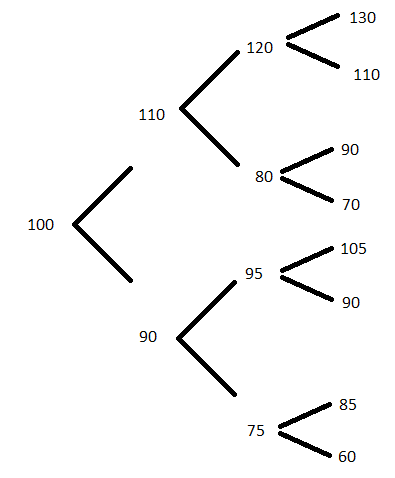
\includegraphics{tree_stock.png}
Suppose the derivative we are pricing is a European call with strike \(95\). At time 3, from top to bottom, the payoffs are 35, 15, 0, 0, 10, 0, 0, and 0. Suppose \(r = 3\%\) and the timestep is \(\Delta_t = 1\) for simplicity. Then, at time 2 at node \(120\), we have \(q = (120 e^{0.03} - 110)/20 = 0.6827\) and \(1-q=0.3173\). The price of the derivative at node 120 is \(e^{-0.03}(0.6827\times 35 + 0.3173 \times 15) = 27.8077\). The price at the 80 node is 0.

Similarly, the price of the derivative at the \(95\) node is \(10e^{-0.03}\cdot q\) where \(q = (95 e^{0.03} - 90)/15 = 0.5262\), yielding a price of \(5.1066\).

Backtracking to the time 1 nodes, we have derivative prices of 22.50 at node 110 and 4.3959 at node 90. Finally, at time 0 (and node 100) we find the price is 15.72579.

\hypertarget{the-geometric-brownian-motion-model-of-asset-value-and-monte-carlo-simulation}{%
\chapter{The geometric Brownian motion model of asset value and Monte Carlo simulation}\label{the-geometric-brownian-motion-model-of-asset-value-and-monte-carlo-simulation}}

\hypertarget{asset-values-as-random-variables}{%
\section{Asset values as random variables}\label{asset-values-as-random-variables}}

Let \(\{S_t, t\geq 0\}\) denote the values of an asset at times \(t\). Ideally, we think of time as a continuum, so that \(S_t\) is a \emph{continuous process}. Practically, however, we will approximate the continuous process by a discrete one by performing computations associated with the process at a grid of \(t\) values in some interval \([0,T]\) with mesh-size \(\Delta t\).

We model the process \(S_t\) as a random or stochastic sequence; essentially, it is just a sequence of realizations of random variables.

Here is a plot of Apple's (AAPL) close-of-day stock price and logarithm of return \(\log(S_t/S_{t-1})\) from its initial listing to the present day. Stock prices are available much more often than daily, so the data visualized below already represent a discretization of the underlying process (with mesh-size 1 day).

\begin{Shaded}
\begin{Highlighting}[]
\ImportTok{import}\NormalTok{ numpy }\ImportTok{as}\NormalTok{ np}
\ImportTok{import}\NormalTok{ numpy.random }\ImportTok{as}\NormalTok{ npr}
\ImportTok{import}\NormalTok{ matplotlib }\ImportTok{as}\NormalTok{ mpl}
\ImportTok{from}\NormalTok{ matplotlib.pylab }\ImportTok{import}\NormalTok{ plt }
\ImportTok{import}\NormalTok{ math}

\NormalTok{plt.style.use(}\StringTok{\textquotesingle{}seaborn\textquotesingle{}}\NormalTok{)}
\NormalTok{mpl.rcParams[}\StringTok{\textquotesingle{}font.family\textquotesingle{}}\NormalTok{] }\OperatorTok{=} \StringTok{\textquotesingle{}serif\textquotesingle{}}

\ImportTok{import}\NormalTok{ pandas }\ImportTok{as}\NormalTok{ pd}
\ImportTok{import}\NormalTok{ yfinance }\ImportTok{as}\NormalTok{ yf}
\ImportTok{from}\NormalTok{ yahoofinancials }\ImportTok{import}\NormalTok{ YahooFinancials}

\NormalTok{aapl\_df }\OperatorTok{=}\NormalTok{ yf.download(}\StringTok{\textquotesingle{}AAPL\textquotesingle{}}\NormalTok{)}
\end{Highlighting}
\end{Shaded}

\begin{verbatim}
## [*********************100%***********************]  1 of 1 completed
\end{verbatim}

\begin{Shaded}
\begin{Highlighting}[]
\NormalTok{close\_price }\OperatorTok{=}\NormalTok{ aapl\_df[}\StringTok{\textquotesingle{}Adj Close\textquotesingle{}}\NormalTok{]}
\NormalTok{log\_rets }\OperatorTok{=}\NormalTok{ np.log(close\_price }\OperatorTok{/}\NormalTok{ close\_price.shift(}\DecValTok{1}\NormalTok{))}
\NormalTok{aapl\_df[}\StringTok{\textquotesingle{}log\_rets\textquotesingle{}}\NormalTok{] }\OperatorTok{=}\NormalTok{ log\_rets}
\NormalTok{aapl\_df[[}\StringTok{\textquotesingle{}Adj Close\textquotesingle{}}\NormalTok{, }\StringTok{\textquotesingle{}log\_rets\textquotesingle{}}\NormalTok{]].plot(subplots}\OperatorTok{=}\VariableTok{True}\NormalTok{, figsize}\OperatorTok{=}\NormalTok{(}\DecValTok{10}\NormalTok{, }\DecValTok{6}\NormalTok{))}
\end{Highlighting}
\end{Shaded}

\begin{verbatim}
## array([<AxesSubplot:xlabel='Date'>, <AxesSubplot:xlabel='Date'>],
##       dtype=object)
\end{verbatim}

\begin{Shaded}
\begin{Highlighting}[]
\NormalTok{plt.show()}\OperatorTok{;}
\end{Highlighting}
\end{Shaded}

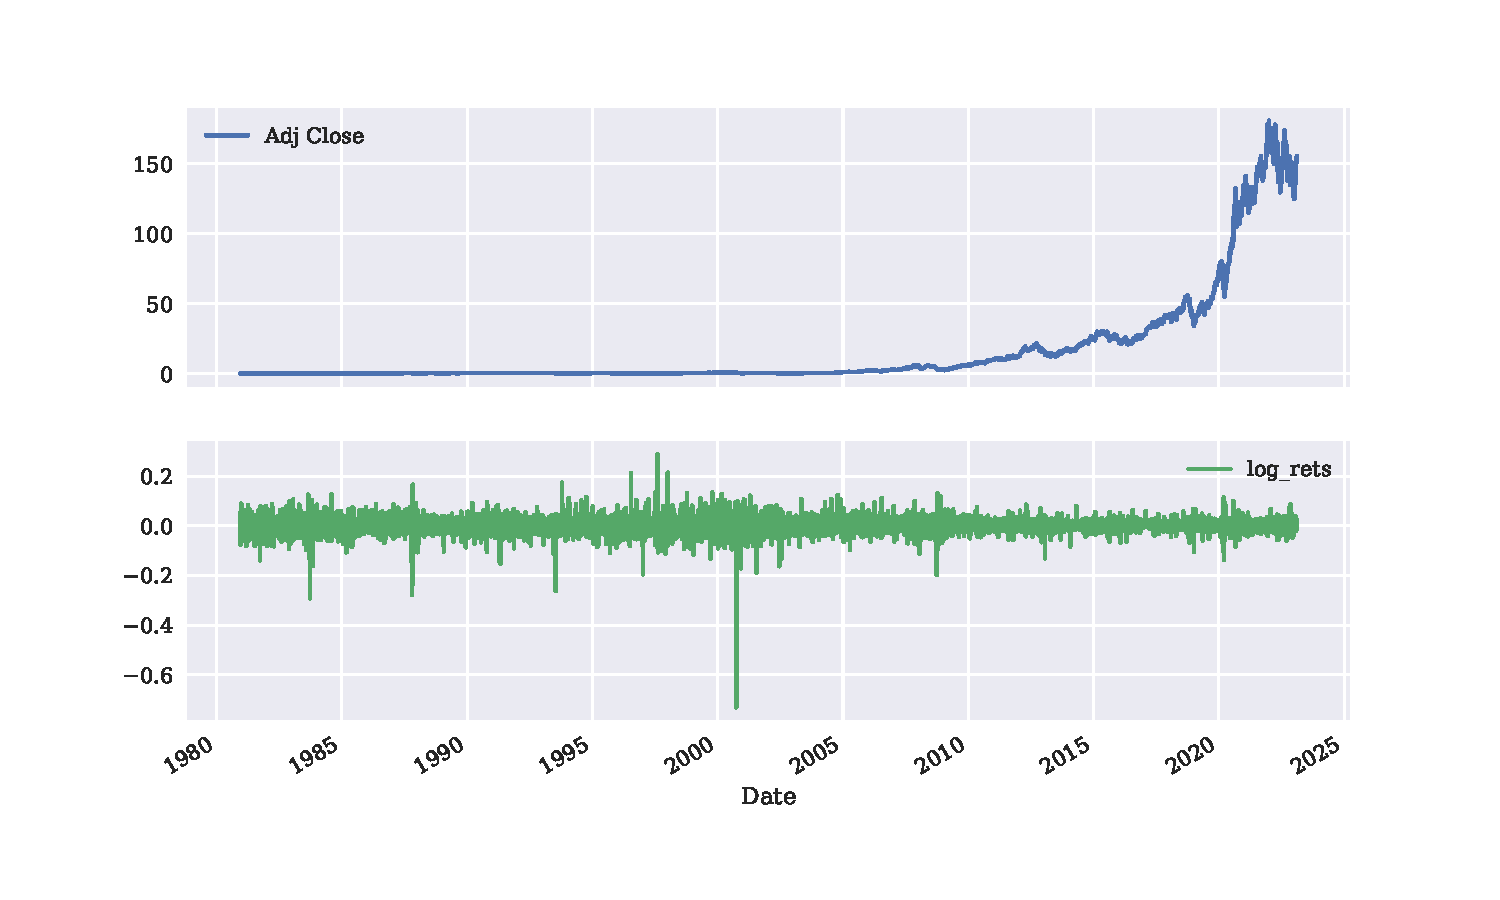
\includegraphics{Financial-Mathematics_files/figure-latex/unnamed-chunk-1-1.pdf}

\hypertarget{geometric-brownian-motion-model-of-asset-prices-over-time}{%
\section{Geometric Brownian motion model of asset prices over time}\label{geometric-brownian-motion-model-of-asset-prices-over-time}}

The mathematics of continuous stochastic processes is advanced. Rather than presenting a full account here we focus on an intermediate level of understanding of one of the most common models used for asset prices. Later we will modify the model to account for several real-life phenomena.

It is folk-wisdom that the log returns of at asset \(\log\frac{S_t}{S_{t-1}}\) are normally-distributed, or, rather, are modeled as such. This comes as a consequence of modeling the sequence of asset prices as a \emph{geometric Brownian motion}.

A Brownian motion (which is also called a Wiener process) is essentially a sequence of normal random variables. Specifically, the process \(W_t\) satisfies
- \(W_0 = 0\)
- \(W_t\) is continuous a.s.
- \(W_t\) has independent increments
- \(W_t - W_s \sim N(0,t-s)\) for \(0\leq s\leq t\)
Additionally, the sequence is measurable with respect to a filtration, an ordered family of sigma-fields (for details see, for example, Resnick's A Probability Path Chapter 10).

The geometric Brownian motion (gBm) model says changes in asset price from time \(t\) to time \(t+s\) are determined by a Brownian motion and a drift. This is typically written in the following fashion as a stochastic differential equation (SDE) with respect to instantaneous price change:
\[dS_t = rS_tdt + \sigma S_t dW_t\]
where \(r\) is a risk-free interest rate, \(dt\) is an instantaneous change in time, \(\sigma\) is a volatility (standard deviation) parameter, and \(W_t\) is a Brownian motion.

It is important to keep in mind the SDE doesn't really mean anything---rather, it is simply notation used to express a stochastic integral in a concise manner. A more meaningful expression of the geometric Brownian motion model is given by the difference equation
\[S_{t+s} = S_t = \int_t^{t+s} rS_u\,du + \int_{t}^{t+s} \sigma S_u \, dW_u.\]
The primary challenge to overcome is how to define integration with respect to the Brownian motion \(W_u\). For various technical reasons, such an integration cannot behave exactly in the same way integration works for real-valued functions, i.e., Riemann integration. A new theory of integration, Ito integration, is needed.

Rather than giving a thorough treatment of Ito's calculus, we will simply provide an informal derivation of Ito's Lemma, which is enough to provide a ``solution'' to the geometric Brownian motion. Let \(f(t,\,S_t)\) be a function of time and asset price at time \(t\). Take a two term Taylor expansion of \(f\) and use the geometric Brownian motion SDE in the chain rule as follows:

\begin{align*}
df &= \frac{\partial f}{\partial t}dt + \frac{\partial f}{\partial S_t}dS_t + \frac{1}{2}\frac{\partial^2 f}{\partial S_t^2}dS_t^2 + \cdots\\
& = \frac{\partial f}{\partial t}dt + \frac{\partial f}{\partial S_t}(rS_tdt + \sigma S_t dW_t) + \frac{1}{2}\frac{\partial^2 f}{\partial S_t^2}(r^2S_t^2dt^2 + 2r\sigma S_t^2 dtdW_t + \sigma^2S_t^2dW_t^2) + \cdots.
\end{align*}

Then, Ito's Lemma says \(dW_t^2 = O(dt)\) and the substitution \(dW_t^2 = dt\) is justified, while the terms \(dt^2\) and \(dt\,dW_t\) are ignorable and may be substituted by zero. The Taylor expansion simplifies, according to Ito, to
\[df = \left(\frac{\partial f}{\partial t} + r S_t\frac{\partial f}{\partial S_t} +\frac{\sigma^2}{2}S_t^2\frac{\partial^2 f}{\partial S_t^2}\right)dt + \sigma\frac{\partial f}{\partial S_t}S_t \,dW_t.\]

Now, let \(f(t,\, S_t):= \log(S_t)\), the log asset price at time \(t\). In that case, we have the following derivatives:
\[\partial f/\partial t = 0\quad \partial f/\partial S_t = 1/S_t \quad \partial^2 f/\partial S_t^2 = -1/S_t^2.\]
Substituting these into the SDE above, we get
\[d\log S_t = r\,dt - \frac{\sigma^2}{2S_t^2}S_t^2\,dt + \frac{\sigma}{S_t}S_t\,dW_t. \]
Next integrate both sides:
\[\log S_t = \log(S_0) + \left(r - \frac{\sigma^2}{2}\right)t + \sigma\, W_t.\]
Exponentiate to obtain\\
\[S_t = S_0\exp\left(rt - \frac{\sigma^2}{2}t+\sigma \, W_t\right).\]
Recall that \(W_t - W_0 := W_t\) has variance \(t\) and see that \(S_t/S_0\) is log-normally distributed with parameters \((r - \sigma^2/2)t\) and \(\sigma\, t^{1/2}\), which means it is right-skewed with mean \(\exp(rt)\) and variance \((\exp(\sigma^2 t)-1)\cdot\exp(2rt)\).

Armed with Ito's Lemma, we have confirmed the folk-wisdom that log-returns from time \(t\) to \(t+s\) are (modeled as) normal random variables with mean \((r - \frac{\sigma^2}{2}) s\) and variance \(\sigma^2 s\). One last minor point: if \(S_t/S_0\) has a lognormal distribution with density \(f\), then the density of \(S_t\) is simply
\[g(s) = S_0^{-1}f(s/S_0),\]
a scaled log-normal. This is helpful, e.g., for comparing the exact distribution of \(S_t\) to MC samples values of \(S_t\), as we do below.

\hypertarget{monte-carlo-simulation-of-the-gbm-model}{%
\section{Monte Carlo simulation of the gBm model}\label{monte-carlo-simulation-of-the-gbm-model}}

As we showed above, there is an exact solution to the geometric Brownian motion SDE---namely, a continuous time random process characterized by independent, normal log-returns over disjoint time periods. Equivalently, given the asset value \(S_0\) at time zero we know \(S_t/S_0\) is log-normally distributed with the parameters given above.

Later, we will modify (complicate) the gBm model to take into account several real-life phenomena including, e.g., time-varying volatility. The augmented models do not necessarily have explicit solutions like the gBm model. Alternatively, we can simulate many times from the model to compute approximate solutions---this is called Monte Carlo. It's not needed for the gBm model, but we will illustrate it here in order to take advantage of the simplified setting of gBm before moving on to more complicated models.

Below we compare three methods for computing \(S_T\) at time \(T\), given \(S_0\), \(\sigma\), and \(r\): the explicit solution due to Ito, a Monte Carlo (MC) simulation from the lognormal distribution, and a MC simulation of \emph{paths} of asset values \(S_s\) for a discretization \(s\in \{s_0 = 0, s_1, \ldots, s_{M+1} = T\}\). All three provide the same answer (in a distributional sense) but the MC procedures contain some additional MC variability (noise) that decreases as the number of simulations increases.

\begin{Shaded}
\begin{Highlighting}[]
\ImportTok{import}\NormalTok{ numpy }\ImportTok{as}\NormalTok{ np}
\ImportTok{import}\NormalTok{ numpy.random }\ImportTok{as}\NormalTok{ npr}
\ImportTok{import}\NormalTok{ matplotlib }\ImportTok{as}\NormalTok{ mpl}
\ImportTok{from}\NormalTok{ matplotlib.pylab }\ImportTok{import}\NormalTok{ plt }
\ImportTok{import}\NormalTok{ math}
\ImportTok{from}\NormalTok{ scipy.stats }\ImportTok{import}\NormalTok{ lognorm}
\NormalTok{plt.style.use(}\StringTok{\textquotesingle{}seaborn\textquotesingle{}}\NormalTok{)}
\NormalTok{mpl.rcParams[}\StringTok{\textquotesingle{}font.family\textquotesingle{}}\NormalTok{] }\OperatorTok{=} \StringTok{\textquotesingle{}serif\textquotesingle{}}


\NormalTok{S0 }\OperatorTok{=} \DecValTok{100}
\NormalTok{r }\OperatorTok{=} \FloatTok{0.05}
\NormalTok{sigma }\OperatorTok{=} \FloatTok{0.25}
\NormalTok{T }\OperatorTok{=} \FloatTok{2.0}

\CommentTok{\# Exact density of ST based on gBm model}
\NormalTok{mu }\OperatorTok{=}\NormalTok{ np.exp((r }\OperatorTok{{-}}\NormalTok{ sigma}\OperatorTok{**}\DecValTok{2}\OperatorTok{/}\DecValTok{2}\NormalTok{)}\OperatorTok{*}\NormalTok{T)}
\NormalTok{s }\OperatorTok{=}\NormalTok{ sigma }\OperatorTok{*}\NormalTok{ math.sqrt(T)}
\NormalTok{x }\OperatorTok{=}\NormalTok{ np.linspace(lognorm.ppf(}\FloatTok{0.001}\NormalTok{, s, scale }\OperatorTok{=}\NormalTok{ mu), lognorm.ppf(}\FloatTok{0.999}\NormalTok{, s, scale }\OperatorTok{=}\NormalTok{ mu), }\DecValTok{1000}\NormalTok{)}


\CommentTok{\# MC sampling of density of ST}
\NormalTok{I}\OperatorTok{=}\DecValTok{10000}
\NormalTok{ST }\OperatorTok{=}\NormalTok{ S0 }\OperatorTok{*}\NormalTok{ np.exp((r}\OperatorTok{{-}}\FloatTok{0.5}\OperatorTok{*}\NormalTok{sigma}\OperatorTok{**}\DecValTok{2}\NormalTok{)}\OperatorTok{*}\NormalTok{T }\OperatorTok{+}\NormalTok{ sigma}\OperatorTok{*}\NormalTok{math.sqrt(T)}\OperatorTok{*}\NormalTok{npr.standard\_normal(I))}


\CommentTok{\# MC sampling of asset price path S0 to ST at 50 equally{-}spaced timepoints}
\NormalTok{M}\OperatorTok{=}\DecValTok{50}
\NormalTok{dt }\OperatorTok{=}\NormalTok{ T }\OperatorTok{/}\NormalTok{ M}
\NormalTok{S }\OperatorTok{=}\NormalTok{ np.zeros((M}\OperatorTok{+}\DecValTok{1}\NormalTok{, I))}
\NormalTok{S[}\DecValTok{0}\NormalTok{] }\OperatorTok{=}\NormalTok{ S0}
\ControlFlowTok{for}\NormalTok{ t }\KeywordTok{in} \BuiltInTok{range}\NormalTok{(}\DecValTok{1}\NormalTok{,M}\OperatorTok{+}\DecValTok{1}\NormalTok{):}
\NormalTok{    S[t]}\OperatorTok{=}\NormalTok{S[t}\OperatorTok{{-}}\DecValTok{1}\NormalTok{]}\OperatorTok{*}\NormalTok{np.exp((r }\OperatorTok{{-}} \FloatTok{0.5}\OperatorTok{*}\NormalTok{sigma}\OperatorTok{**}\DecValTok{2}\NormalTok{)}\OperatorTok{*}\NormalTok{dt }\OperatorTok{+}\NormalTok{ sigma}\OperatorTok{*}\NormalTok{math.sqrt(dt)}\OperatorTok{*}\NormalTok{npr.standard\_normal(I))}


\CommentTok{\# Plots of asset Price distribution at T = 2}
\NormalTok{plt.figure(figsize }\OperatorTok{=}\NormalTok{ (}\DecValTok{10}\NormalTok{,}\DecValTok{6}\NormalTok{))}
\NormalTok{plt.subplot(}\DecValTok{211}\NormalTok{)}
\CommentTok{\# histogram of MC samples from scaled log{-}normal}
\NormalTok{hist1 }\OperatorTok{=}\NormalTok{ plt.hist(ST,}\DecValTok{100}\NormalTok{,density }\OperatorTok{=} \VariableTok{True}\NormalTok{)}
\CommentTok{\# scaled log{-}normal density}
\NormalTok{dens }\OperatorTok{=}\NormalTok{ plt.plot(x}\OperatorTok{*}\NormalTok{S0, (}\DecValTok{1}\OperatorTok{/}\NormalTok{S0)}\OperatorTok{*}\NormalTok{lognorm.pdf(x, s, scale }\OperatorTok{=}\NormalTok{ mu),}
       \StringTok{\textquotesingle{}r{-}\textquotesingle{}}\NormalTok{, lw}\OperatorTok{=}\DecValTok{2}\NormalTok{, alpha}\OperatorTok{=}\FloatTok{0.6}\NormalTok{)}
\NormalTok{plt.ylabel(}\StringTok{\textquotesingle{}Asset Price\textquotesingle{}}\NormalTok{)}
\NormalTok{plt.title(}\StringTok{\textquotesingle{}Exact and MC{-}simulated Asset Price at Time T=2\textquotesingle{}}\NormalTok{)}
\NormalTok{plt.xlim([}\DecValTok{0}\NormalTok{,}\DecValTok{400}\NormalTok{])}
\CommentTok{\#plt.ylim([0,0.0014])}
\end{Highlighting}
\end{Shaded}

\begin{verbatim}
## (0.0, 400.0)
\end{verbatim}

\begin{Shaded}
\begin{Highlighting}[]
\NormalTok{plt.subplot(}\DecValTok{212}\NormalTok{)}
\CommentTok{\# histogram of path{-}wise MC samples from scaled log{-}normal over grid of 50 times}
\NormalTok{hist2 }\OperatorTok{=}\NormalTok{ plt.hist(S[}\OperatorTok{{-}}\DecValTok{1}\NormalTok{],}\DecValTok{100}\NormalTok{,density }\OperatorTok{=} \VariableTok{True}\NormalTok{)}
\NormalTok{dens }\OperatorTok{=}\NormalTok{ plt.plot(x}\OperatorTok{*}\NormalTok{S0, (}\DecValTok{1}\OperatorTok{/}\NormalTok{S0)}\OperatorTok{*}\NormalTok{lognorm.pdf(x, s, scale }\OperatorTok{=}\NormalTok{ mu),}
       \StringTok{\textquotesingle{}r{-}\textquotesingle{}}\NormalTok{, lw}\OperatorTok{=}\DecValTok{2}\NormalTok{, alpha}\OperatorTok{=}\FloatTok{0.6}\NormalTok{)}
\NormalTok{plt.ylabel(}\StringTok{\textquotesingle{}Asset Price\textquotesingle{}}\NormalTok{)}
\NormalTok{plt.xlabel(}\StringTok{\textquotesingle{}Time\textquotesingle{}}\NormalTok{)}
\NormalTok{plt.xlim([}\DecValTok{0}\NormalTok{,}\DecValTok{400}\NormalTok{])}
\CommentTok{\#plt.ylim([0,0.0014])}
\end{Highlighting}
\end{Shaded}

\begin{verbatim}
## (0.0, 400.0)
\end{verbatim}

\begin{Shaded}
\begin{Highlighting}[]
\NormalTok{plt.show()}
\end{Highlighting}
\end{Shaded}

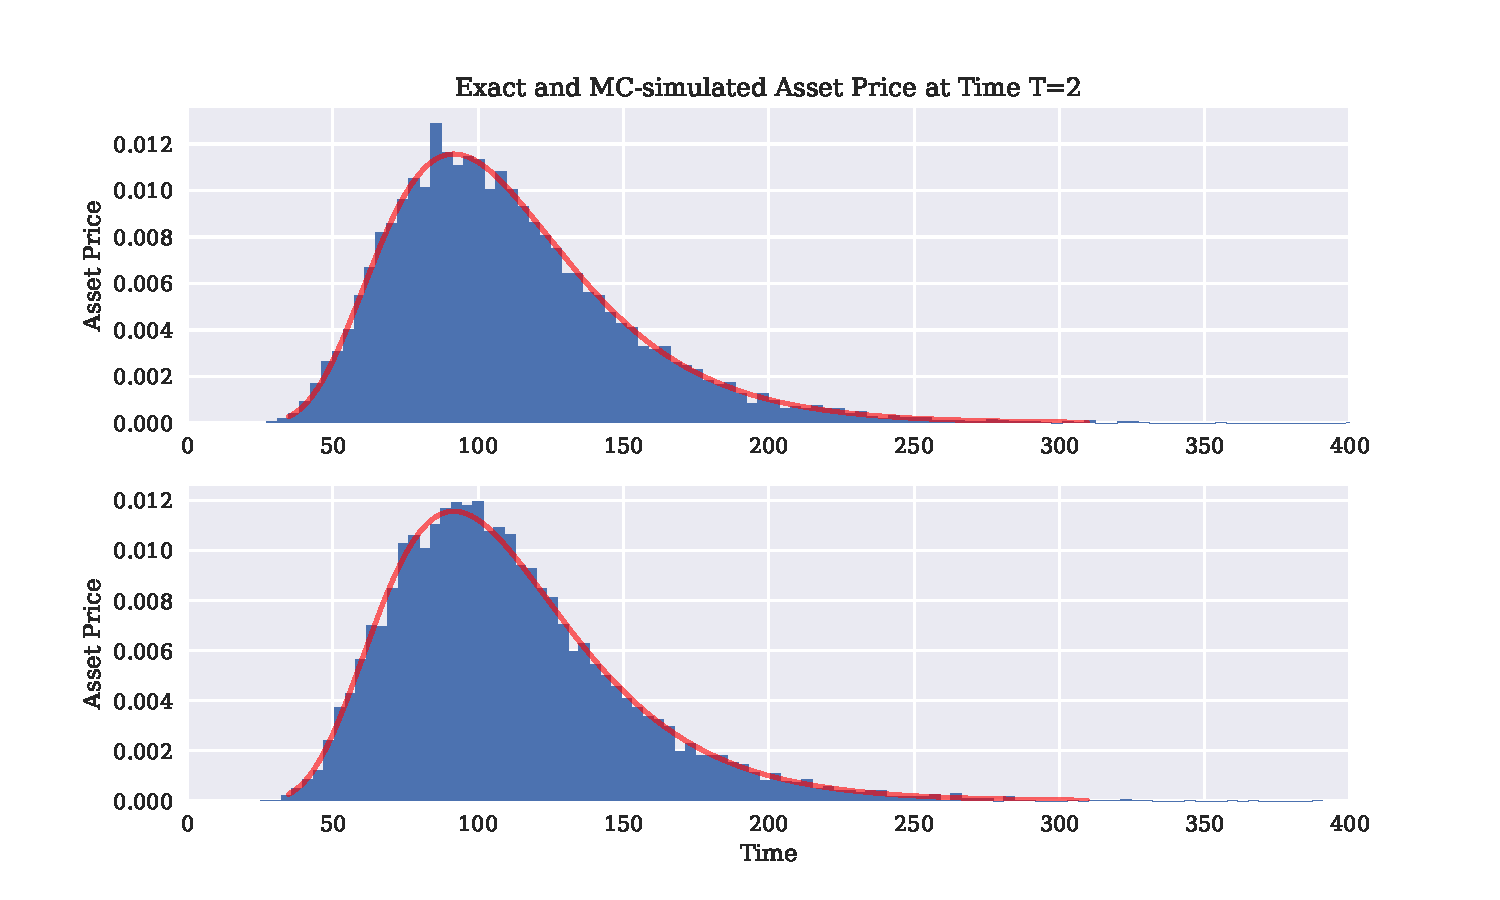
\includegraphics{Financial-Mathematics_files/figure-latex/unnamed-chunk-2-3.pdf}

\hypertarget{off-on-a-tangent-reducing-mc-variability}{%
\section{Off on a tangent: reducing MC variability}\label{off-on-a-tangent-reducing-mc-variability}}

The difference between the theoretic (exact) values for the mean and standard deviation of \(S_T\) and the corresponding MC approximations (shown below) is due to MC error. The Law of Large Numbers (LLN) implies MC error declines to zero as the number of MC samples increases to infinity. In practice, using many more MC samples in order to reduce MC error has the trade-off of increasing computation time (and memory usage if storing those random variates in a vector). On the other hand, there are a few ways to reduce MC error by making more clever choices of MC samples.

\begin{Shaded}
\begin{Highlighting}[]
\ImportTok{import}\NormalTok{ scipy.stats  }\ImportTok{as}\NormalTok{ scs}

\KeywordTok{def}\NormalTok{ print\_stats(a2,a3):}
\NormalTok{    stat2 }\OperatorTok{=}\NormalTok{ scs.describe(a2)}
\NormalTok{    stat3 }\OperatorTok{=}\NormalTok{ scs.describe(a3)}
    \BuiltInTok{print}\NormalTok{(}\StringTok{\textquotesingle{}}\SpecialCharTok{\%14s}\StringTok{ }\SpecialCharTok{\%14s}\StringTok{ }\SpecialCharTok{\%14s}\StringTok{ }\SpecialCharTok{\%14s}\StringTok{\textquotesingle{}} \OperatorTok{\%}\NormalTok{ (}\StringTok{\textquotesingle{}statistic\textquotesingle{}}\NormalTok{, }\StringTok{\textquotesingle{}data set 1\textquotesingle{}}\NormalTok{, }\StringTok{\textquotesingle{}data set 2\textquotesingle{}}\NormalTok{, }\StringTok{\textquotesingle{}data set 3\textquotesingle{}}\NormalTok{))}
    \BuiltInTok{print}\NormalTok{(}\DecValTok{45} \OperatorTok{*} \StringTok{\textquotesingle{}{-}\textquotesingle{}}\NormalTok{)}
    \BuiltInTok{print}\NormalTok{(}\StringTok{\textquotesingle{}}\SpecialCharTok{\%14s}\StringTok{ }\SpecialCharTok{\%14s}\StringTok{ }\SpecialCharTok{\%14.3f}\StringTok{ }\SpecialCharTok{\%14.3f}\StringTok{\textquotesingle{}} \OperatorTok{\%}\NormalTok{ (}\StringTok{\textquotesingle{}size\textquotesingle{}}\NormalTok{, }\StringTok{\textquotesingle{}NA\textquotesingle{}}\NormalTok{, stat2[}\DecValTok{0}\NormalTok{], stat3[}\DecValTok{0}\NormalTok{]))}
    \BuiltInTok{print}\NormalTok{(}\StringTok{\textquotesingle{}}\SpecialCharTok{\%14s}\StringTok{ }\SpecialCharTok{\%14s}\StringTok{ }\SpecialCharTok{\%14.3f}\StringTok{ }\SpecialCharTok{\%14.3f}\StringTok{\textquotesingle{}} \OperatorTok{\%}\NormalTok{ (}\StringTok{\textquotesingle{}min\textquotesingle{}}\NormalTok{, }\StringTok{\textquotesingle{}NA\textquotesingle{}}\NormalTok{, stat2[}\DecValTok{1}\NormalTok{][}\DecValTok{0}\NormalTok{], stat3[}\DecValTok{1}\NormalTok{][}\DecValTok{0}\NormalTok{] ))}
    \BuiltInTok{print}\NormalTok{(}\StringTok{\textquotesingle{}}\SpecialCharTok{\%14s}\StringTok{ }\SpecialCharTok{\%14s}\StringTok{ }\SpecialCharTok{\%14.3f}\StringTok{ }\SpecialCharTok{\%14.3f}\StringTok{\textquotesingle{}} \OperatorTok{\%}\NormalTok{ (}\StringTok{\textquotesingle{}max\textquotesingle{}}\NormalTok{, }\StringTok{\textquotesingle{}NA\textquotesingle{}}\NormalTok{, stat2[}\DecValTok{1}\NormalTok{][}\DecValTok{1}\NormalTok{], stat3[}\DecValTok{1}\NormalTok{][}\DecValTok{1}\NormalTok{]))}
    \BuiltInTok{print}\NormalTok{(}\StringTok{\textquotesingle{}}\SpecialCharTok{\%14s}\StringTok{ }\SpecialCharTok{\%14.3f}\StringTok{ }\SpecialCharTok{\%14.3f}\StringTok{ }\SpecialCharTok{\%14.3f}\StringTok{\textquotesingle{}} \OperatorTok{\%}\NormalTok{ (}\StringTok{\textquotesingle{}mean\textquotesingle{}}\NormalTok{, S0}\OperatorTok{*}\NormalTok{math.exp(r}\OperatorTok{*}\NormalTok{T), stat2[}\DecValTok{2}\NormalTok{], stat3[}\DecValTok{2}\NormalTok{]))}
    \BuiltInTok{print}\NormalTok{(}\StringTok{\textquotesingle{}}\SpecialCharTok{\%14s}\StringTok{ }\SpecialCharTok{\%14.3f}\StringTok{ }\SpecialCharTok{\%14.3f}\StringTok{ }\SpecialCharTok{\%14.3f}\StringTok{\textquotesingle{}} \OperatorTok{\%}\NormalTok{ (}\StringTok{\textquotesingle{}stdev\textquotesingle{}}\NormalTok{, S0}\OperatorTok{*}\NormalTok{math.sqrt((math.exp(sigma}\OperatorTok{**}\DecValTok{2} \OperatorTok{*}\NormalTok{ T)}\OperatorTok{{-}}\DecValTok{1}\NormalTok{)}\OperatorTok{*}\NormalTok{math.exp(}\DecValTok{2}\OperatorTok{*}\NormalTok{r}\OperatorTok{*}\NormalTok{T)), np.sqrt(stat2[}\DecValTok{3}\NormalTok{]), np.sqrt(stat3[}\DecValTok{3}\NormalTok{])))}


\NormalTok{print\_stats(ST, S[}\OperatorTok{{-}}\DecValTok{1}\NormalTok{])}
\end{Highlighting}
\end{Shaded}

\begin{verbatim}
##      statistic     data set 1     data set 2     data set 3
## ---------------------------------------------
##           size             NA      10000.000      10000.000
##            min             NA         27.396         26.587
##            max             NA        368.480        365.911
##           mean        110.517        109.556        110.735
##          stdev         40.327         39.776         39.986
\end{verbatim}

The simplest way to reduce MC variability (besides increasing the number of samples) is to use \emph{anti-thetical variates}. When sampling standard normal random variates this amounts to sampling \(z\) and using both \((z,-z)\) as samples. To get \(2I\) samples one only needs to actually compute \(I\) samples, the remaining \(I\) are the same in magnitude but with the opposite signs. This accomplishes exact mean-matching, i.e., \((2I)^{-1}\sum_{i=1}^{2I} z_i = 0\), exactly the standard normal distribution mean.

Another method for reducing MC variability is second-moment matching. Suppose we generate antithetical samples \(z = (z_1, \ldots, z_I)\). Let \(z^\star_i := z_i / s_{z}\) for \(i=1, \ldots, I\) where \(s_z\) is the sample standard deviation of \(z\). Now, \(z^\star\) has sample mean exactly zero and sample standard deviation exactly \(1\).

Further, a Box-Cox transformation may be used if the samples \(z\) have positive skew. (If they have negative skew, then the samples may be reflected about the maximum value to produce a set of positively-skewed values starting from zero.) After applying the Box-cox transformation, the resulting values \(y\) should be close to symmetric (closer to a normal distribution than the original variates) and a further standardization \(z^\star_i = (y_i - \overline y)/s_y\) may be used to transform the values to approximately standard normal.

The following simulation supports the use of standardized antithetic variates. By design, these had exactly zero mean and unit variance, but were slightly more likely to be skewed compared to vanilly MC samples. Box-Cox transformed variates did not perform better, and were more likely to display excess kurtosis than even vanilla MC variates. It is worth pointing out that antithetic variates may be produced sequentially while standardized variates requires storing all variates in memory, which may be a problem in some applications.

\begin{Shaded}
\begin{Highlighting}[]
\ImportTok{import}\NormalTok{ scipy.stats  }\ImportTok{as}\NormalTok{ scs}
\ImportTok{import}\NormalTok{ numpy  }\ImportTok{as}\NormalTok{ np}
\ImportTok{import}\NormalTok{ numpy.random  }\ImportTok{as}\NormalTok{ npr}

\KeywordTok{def}\NormalTok{ bc\_standardize(z):}
\NormalTok{  M }\OperatorTok{=}\NormalTok{ np.}\BuiltInTok{max}\NormalTok{(z)}
\NormalTok{  zM }\OperatorTok{=}\NormalTok{ M}\OperatorTok{{-}}\NormalTok{z}\OperatorTok{+}\FloatTok{0.0000001}
\NormalTok{  y }\OperatorTok{=}\NormalTok{ scs.boxcox(zM)}
\NormalTok{  m }\OperatorTok{=}\NormalTok{ np.mean(y[}\DecValTok{0}\NormalTok{])}
\NormalTok{  s }\OperatorTok{=}\NormalTok{ np.std(y[}\DecValTok{0}\NormalTok{], ddof}\OperatorTok{=}\DecValTok{1}\NormalTok{)}
\NormalTok{  z\_star }\OperatorTok{=}\NormalTok{ (y[}\DecValTok{0}\NormalTok{]}\OperatorTok{{-}}\NormalTok{m)}\OperatorTok{/}\NormalTok{s}
  \ControlFlowTok{return}\NormalTok{ z\_star}

\KeywordTok{def}\NormalTok{ at\_standardize(z):}
\NormalTok{  s }\OperatorTok{=}\NormalTok{ np.std(z, ddof}\OperatorTok{=}\DecValTok{1}\NormalTok{)}
\NormalTok{  z\_star }\OperatorTok{=}\NormalTok{ z}\OperatorTok{/}\NormalTok{s}
  \ControlFlowTok{return}\NormalTok{ z\_star}

\NormalTok{kurtosis\_vals }\OperatorTok{=}\NormalTok{ np.zeros((}\DecValTok{1000}\NormalTok{,}\DecValTok{8}\NormalTok{))}
\NormalTok{skew\_vals }\OperatorTok{=}\NormalTok{ np.zeros\_like(kurtosis\_vals)}
\NormalTok{mean\_vals }\OperatorTok{=}\NormalTok{ np.zeros\_like(kurtosis\_vals)}
\NormalTok{std\_vals }\OperatorTok{=}\NormalTok{ np.zeros\_like(kurtosis\_vals)}

\KeywordTok{def}\NormalTok{ print\_stats2():}
  \ControlFlowTok{for}\NormalTok{ i }\KeywordTok{in} \BuiltInTok{range}\NormalTok{(}\DecValTok{1}\NormalTok{,}\DecValTok{1001}\NormalTok{):}
\NormalTok{    X }\OperatorTok{=}\NormalTok{ npr.standard\_normal(}\DecValTok{10000}\NormalTok{)}
\NormalTok{    Z1 }\OperatorTok{=}\NormalTok{ npr.standard\_normal(}\DecValTok{5000}\NormalTok{)}
\NormalTok{    Z2 }\OperatorTok{=}\NormalTok{ npr.standard\_normal(}\DecValTok{5000}\NormalTok{)}
\NormalTok{    Z3 }\OperatorTok{=} \OperatorTok{{-}}\NormalTok{Z1}
\NormalTok{    Z4 }\OperatorTok{=} \OperatorTok{{-}}\NormalTok{Z2}
\NormalTok{    Z }\OperatorTok{=}\NormalTok{ np.concatenate((Z1,Z2))}
\NormalTok{    Y }\OperatorTok{=}\NormalTok{ np.concatenate((Z1,Z3))}
\NormalTok{    W }\OperatorTok{=}\NormalTok{ np.concatenate((Z2,Z4))}
\NormalTok{    Ystar }\OperatorTok{=}\NormalTok{ bc\_standardize(Y)}
\NormalTok{    Wstar }\OperatorTok{=}\NormalTok{ bc\_standardize(W)}
\NormalTok{    Yst }\OperatorTok{=}\NormalTok{ at\_standardize(Y)}
\NormalTok{    Wst }\OperatorTok{=}\NormalTok{ at\_standardize(W)}
\NormalTok{    stat1 }\OperatorTok{=}\NormalTok{ scs.describe(X, ddof }\OperatorTok{=} \DecValTok{1}\NormalTok{)}
\NormalTok{    stat2 }\OperatorTok{=}\NormalTok{ scs.describe(Z, ddof }\OperatorTok{=} \DecValTok{1}\NormalTok{)}
\NormalTok{    stat3 }\OperatorTok{=}\NormalTok{ scs.describe(Y, ddof }\OperatorTok{=} \DecValTok{1}\NormalTok{)}
\NormalTok{    stat4 }\OperatorTok{=}\NormalTok{ scs.describe(W, ddof }\OperatorTok{=} \DecValTok{1}\NormalTok{)}
\NormalTok{    stat5 }\OperatorTok{=}\NormalTok{ scs.describe(Ystar, ddof }\OperatorTok{=} \DecValTok{1}\NormalTok{)}
\NormalTok{    stat6 }\OperatorTok{=}\NormalTok{ scs.describe(Wstar, ddof }\OperatorTok{=} \DecValTok{1}\NormalTok{)}
\NormalTok{    stat7 }\OperatorTok{=}\NormalTok{ scs.describe(Yst, ddof }\OperatorTok{=} \DecValTok{1}\NormalTok{)}
\NormalTok{    stat8 }\OperatorTok{=}\NormalTok{ scs.describe(Wst, ddof }\OperatorTok{=} \DecValTok{1}\NormalTok{)}
\NormalTok{    mean\_vals[i}\OperatorTok{{-}}\DecValTok{1}\NormalTok{,:] }\OperatorTok{=}\NormalTok{ np.array([stat1[}\DecValTok{2}\NormalTok{], stat2[}\DecValTok{2}\NormalTok{], stat3[}\DecValTok{2}\NormalTok{], stat4[}\DecValTok{2}\NormalTok{], stat5[}\DecValTok{2}\NormalTok{], stat6[}\DecValTok{2}\NormalTok{], stat7[}\DecValTok{2}\NormalTok{], stat8[}\DecValTok{2}\NormalTok{]])}
\NormalTok{    std\_vals[i}\OperatorTok{{-}}\DecValTok{1}\NormalTok{,:] }\OperatorTok{=}\NormalTok{ np.array([stat1[}\DecValTok{3}\NormalTok{], stat2[}\DecValTok{3}\NormalTok{], stat3[}\DecValTok{3}\NormalTok{], stat4[}\DecValTok{3}\NormalTok{], stat5[}\DecValTok{3}\NormalTok{], stat6[}\DecValTok{3}\NormalTok{], stat7[}\DecValTok{3}\NormalTok{], stat8[}\DecValTok{3}\NormalTok{]])}
\NormalTok{    kurtosis\_vals[i}\OperatorTok{{-}}\DecValTok{1}\NormalTok{,:] }\OperatorTok{=}\NormalTok{ np.array([stat1[}\DecValTok{4}\NormalTok{], stat2[}\DecValTok{4}\NormalTok{], stat3[}\DecValTok{4}\NormalTok{], stat4[}\DecValTok{4}\NormalTok{], stat5[}\DecValTok{4}\NormalTok{], stat6[}\DecValTok{4}\NormalTok{], stat7[}\DecValTok{4}\NormalTok{], stat8[}\DecValTok{4}\NormalTok{]])}
\NormalTok{    skew\_vals[i}\OperatorTok{{-}}\DecValTok{1}\NormalTok{,:] }\OperatorTok{=}\NormalTok{ np.array([stat1[}\DecValTok{5}\NormalTok{], stat2[}\DecValTok{5}\NormalTok{], stat3[}\DecValTok{5}\NormalTok{], stat4[}\DecValTok{5}\NormalTok{], stat5[}\DecValTok{5}\NormalTok{], stat6[}\DecValTok{5}\NormalTok{], stat7[}\DecValTok{5}\NormalTok{], stat8[}\DecValTok{5}\NormalTok{]])}

  \BuiltInTok{print}\NormalTok{(}\StringTok{\textquotesingle{}}\SpecialCharTok{\%14s}\StringTok{ }\SpecialCharTok{\%14s}\StringTok{ }\SpecialCharTok{\%14s}\StringTok{ }\SpecialCharTok{\%14s}\StringTok{ }\SpecialCharTok{\%14s}\StringTok{ }\SpecialCharTok{\%14s}\StringTok{ }\SpecialCharTok{\%14s}\StringTok{ }\SpecialCharTok{\%14s}\StringTok{ }\SpecialCharTok{\%14s}\StringTok{\textquotesingle{}} \OperatorTok{\%}\NormalTok{ (}\StringTok{\textquotesingle{}statistic\textquotesingle{}}\NormalTok{, }\StringTok{\textquotesingle{}data set 1\textquotesingle{}}\NormalTok{, }\StringTok{\textquotesingle{}data set 2\textquotesingle{}}\NormalTok{, }\StringTok{\textquotesingle{}data set 3\textquotesingle{}}\NormalTok{, }\StringTok{\textquotesingle{}data set 4\textquotesingle{}}\NormalTok{, }\StringTok{\textquotesingle{}data set 5\textquotesingle{}}\NormalTok{, }\StringTok{\textquotesingle{}data set 6\textquotesingle{}}\NormalTok{, }\StringTok{\textquotesingle{}data set 7\textquotesingle{}}\NormalTok{, }\StringTok{\textquotesingle{}data set 8\textquotesingle{}}\NormalTok{))}
  \BuiltInTok{print}\NormalTok{(}\StringTok{\textquotesingle{}}\SpecialCharTok{\%14s}\StringTok{ }\SpecialCharTok{\%14.3f}\StringTok{ }\SpecialCharTok{\%14.3f}\StringTok{ }\SpecialCharTok{\%14.3f}\StringTok{ }\SpecialCharTok{\%14.3f}\StringTok{ }\SpecialCharTok{\%14.3f}\StringTok{ }\SpecialCharTok{\%14.3f}\StringTok{ }\SpecialCharTok{\%14.3f}\StringTok{ }\SpecialCharTok{\%14.3f}\StringTok{\textquotesingle{}} \OperatorTok{\%}\NormalTok{ (}\StringTok{\textquotesingle{}mean mean\textquotesingle{}}\NormalTok{, np.mean(mean\_vals[:,}\DecValTok{0}\NormalTok{]), np.mean(mean\_vals[:,}\DecValTok{1}\NormalTok{]), np.mean(mean\_vals[:,}\DecValTok{2}\NormalTok{]), np.mean(mean\_vals[:,}\DecValTok{3}\NormalTok{]), np.mean(mean\_vals[:,}\DecValTok{4}\NormalTok{]), np.mean(mean\_vals[:,}\DecValTok{5}\NormalTok{]), np.mean(mean\_vals[:,}\DecValTok{6}\NormalTok{]), np.mean(mean\_vals[:,}\DecValTok{7}\NormalTok{])))}
  \BuiltInTok{print}\NormalTok{(}\StringTok{\textquotesingle{}}\SpecialCharTok{\%14s}\StringTok{ }\SpecialCharTok{\%14.3f}\StringTok{ }\SpecialCharTok{\%14.3f}\StringTok{ }\SpecialCharTok{\%14.3f}\StringTok{ }\SpecialCharTok{\%14.3f}\StringTok{ }\SpecialCharTok{\%14.3f}\StringTok{ }\SpecialCharTok{\%14.3f}\StringTok{ }\SpecialCharTok{\%14.3f}\StringTok{ }\SpecialCharTok{\%14.3f}\StringTok{\textquotesingle{}} \OperatorTok{\%}\NormalTok{ (}\StringTok{\textquotesingle{}std mean\textquotesingle{}}\NormalTok{, np.std(mean\_vals[:,}\DecValTok{0}\NormalTok{]), np.std(mean\_vals[:,}\DecValTok{1}\NormalTok{]), np.std(mean\_vals[:,}\DecValTok{2}\NormalTok{]), np.std(mean\_vals[:,}\DecValTok{3}\NormalTok{]), np.std(mean\_vals[:,}\DecValTok{4}\NormalTok{]), np.std(mean\_vals[:,}\DecValTok{5}\NormalTok{]), np.std(mean\_vals[:,}\DecValTok{6}\NormalTok{]), np.std(mean\_vals[:,}\DecValTok{7}\NormalTok{])))}
  \BuiltInTok{print}\NormalTok{(}\StringTok{\textquotesingle{}}\SpecialCharTok{\%14s}\StringTok{ }\SpecialCharTok{\%14.3f}\StringTok{ }\SpecialCharTok{\%14.3f}\StringTok{ }\SpecialCharTok{\%14.3f}\StringTok{ }\SpecialCharTok{\%14.3f}\StringTok{ }\SpecialCharTok{\%14.3f}\StringTok{ }\SpecialCharTok{\%14.3f}\StringTok{ }\SpecialCharTok{\%14.3f}\StringTok{ }\SpecialCharTok{\%14.3f}\StringTok{\textquotesingle{}} \OperatorTok{\%}\NormalTok{ (}\StringTok{\textquotesingle{}mean std\textquotesingle{}}\NormalTok{, np.mean(std\_vals[:,}\DecValTok{0}\NormalTok{]), np.mean(std\_vals[:,}\DecValTok{1}\NormalTok{]), np.mean(std\_vals[:,}\DecValTok{2}\NormalTok{]), np.mean(std\_vals[:,}\DecValTok{3}\NormalTok{]), np.mean(std\_vals[:,}\DecValTok{4}\NormalTok{]), np.mean(std\_vals[:,}\DecValTok{5}\NormalTok{]), np.mean(std\_vals[:,}\DecValTok{6}\NormalTok{]), np.mean(std\_vals[:,}\DecValTok{7}\NormalTok{])))}
  \BuiltInTok{print}\NormalTok{(}\StringTok{\textquotesingle{}}\SpecialCharTok{\%14s}\StringTok{ }\SpecialCharTok{\%14.3f}\StringTok{ }\SpecialCharTok{\%14.3f}\StringTok{ }\SpecialCharTok{\%14.3f}\StringTok{ }\SpecialCharTok{\%14.3f}\StringTok{ }\SpecialCharTok{\%14.3f}\StringTok{ }\SpecialCharTok{\%14.3f}\StringTok{ }\SpecialCharTok{\%14.3f}\StringTok{ }\SpecialCharTok{\%14.3f}\StringTok{\textquotesingle{}} \OperatorTok{\%}\NormalTok{ (}\StringTok{\textquotesingle{}std std\textquotesingle{}}\NormalTok{, np.std(std\_vals[:,}\DecValTok{0}\NormalTok{]), np.std(std\_vals[:,}\DecValTok{1}\NormalTok{]), np.std(std\_vals[:,}\DecValTok{2}\NormalTok{]), np.std(std\_vals[:,}\DecValTok{3}\NormalTok{]), np.std(std\_vals[:,}\DecValTok{4}\NormalTok{]), np.std(std\_vals[:,}\DecValTok{5}\NormalTok{]), np.std(std\_vals[:,}\DecValTok{6}\NormalTok{]), np.std(std\_vals[:,}\DecValTok{7}\NormalTok{])))}
  \BuiltInTok{print}\NormalTok{(}\StringTok{\textquotesingle{}}\SpecialCharTok{\%14s}\StringTok{ }\SpecialCharTok{\%14.3f}\StringTok{ }\SpecialCharTok{\%14.3f}\StringTok{ }\SpecialCharTok{\%14.3f}\StringTok{ }\SpecialCharTok{\%14.3f}\StringTok{ }\SpecialCharTok{\%14.3f}\StringTok{ }\SpecialCharTok{\%14.3f}\StringTok{ }\SpecialCharTok{\%14.3f}\StringTok{ }\SpecialCharTok{\%14.3f}\StringTok{\textquotesingle{}} \OperatorTok{\%}\NormalTok{ (}\StringTok{\textquotesingle{}mean kurtosis\textquotesingle{}}\NormalTok{, np.mean(kurtosis\_vals[:,}\DecValTok{0}\NormalTok{]), np.mean(kurtosis\_vals[:,}\DecValTok{1}\NormalTok{]), np.mean(kurtosis\_vals[:,}\DecValTok{2}\NormalTok{]), np.mean(kurtosis\_vals[:,}\DecValTok{3}\NormalTok{]), np.mean(kurtosis\_vals[:,}\DecValTok{4}\NormalTok{]), np.mean(kurtosis\_vals[:,}\DecValTok{5}\NormalTok{]), np.mean(kurtosis\_vals[:,}\DecValTok{6}\NormalTok{]), np.mean(kurtosis\_vals[:,}\DecValTok{7}\NormalTok{])))}
  \BuiltInTok{print}\NormalTok{(}\StringTok{\textquotesingle{}}\SpecialCharTok{\%14s}\StringTok{ }\SpecialCharTok{\%14.3f}\StringTok{ }\SpecialCharTok{\%14.3f}\StringTok{ }\SpecialCharTok{\%14.3f}\StringTok{ }\SpecialCharTok{\%14.3f}\StringTok{ }\SpecialCharTok{\%14.3f}\StringTok{ }\SpecialCharTok{\%14.3f}\StringTok{ }\SpecialCharTok{\%14.3f}\StringTok{ }\SpecialCharTok{\%14.3f}\StringTok{\textquotesingle{}} \OperatorTok{\%}\NormalTok{ (}\StringTok{\textquotesingle{}std kurtosis\textquotesingle{}}\NormalTok{, np.std(kurtosis\_vals[:,}\DecValTok{0}\NormalTok{]), np.std(kurtosis\_vals[:,}\DecValTok{1}\NormalTok{]), np.std(kurtosis\_vals[:,}\DecValTok{2}\NormalTok{]), np.std(kurtosis\_vals[:,}\DecValTok{3}\NormalTok{]), np.std(kurtosis\_vals[:,}\DecValTok{4}\NormalTok{]), np.std(kurtosis\_vals[:,}\DecValTok{5}\NormalTok{]), np.std(kurtosis\_vals[:,}\DecValTok{6}\NormalTok{]), np.std(kurtosis\_vals[:,}\DecValTok{7}\NormalTok{])))}
  \BuiltInTok{print}\NormalTok{(}\StringTok{\textquotesingle{}}\SpecialCharTok{\%14s}\StringTok{ }\SpecialCharTok{\%14.3f}\StringTok{ }\SpecialCharTok{\%14.3f}\StringTok{ }\SpecialCharTok{\%14.3f}\StringTok{ }\SpecialCharTok{\%14.3f}\StringTok{ }\SpecialCharTok{\%14.3f}\StringTok{ }\SpecialCharTok{\%14.3f}\StringTok{ }\SpecialCharTok{\%14.3f}\StringTok{ }\SpecialCharTok{\%14.3f}\StringTok{\textquotesingle{}} \OperatorTok{\%}\NormalTok{ (}\StringTok{\textquotesingle{}mean skew\textquotesingle{}}\NormalTok{, np.mean(skew\_vals[:,}\DecValTok{0}\NormalTok{]), np.mean(skew\_vals[:,}\DecValTok{1}\NormalTok{]), np.mean(skew\_vals[:,}\DecValTok{2}\NormalTok{]), np.mean(skew\_vals[:,}\DecValTok{3}\NormalTok{]), np.mean(skew\_vals[:,}\DecValTok{4}\NormalTok{]), np.mean(skew\_vals[:,}\DecValTok{5}\NormalTok{]), np.mean(skew\_vals[:,}\DecValTok{6}\NormalTok{]), np.mean(skew\_vals[:,}\DecValTok{7}\NormalTok{])))}
  \BuiltInTok{print}\NormalTok{(}\StringTok{\textquotesingle{}}\SpecialCharTok{\%14s}\StringTok{ }\SpecialCharTok{\%14.3f}\StringTok{ }\SpecialCharTok{\%14.3f}\StringTok{ }\SpecialCharTok{\%14.3f}\StringTok{ }\SpecialCharTok{\%14.3f}\StringTok{ }\SpecialCharTok{\%14.3f}\StringTok{ }\SpecialCharTok{\%14.3f}\StringTok{ }\SpecialCharTok{\%14.3f}\StringTok{ }\SpecialCharTok{\%14.3f}\StringTok{\textquotesingle{}} \OperatorTok{\%}\NormalTok{ (}\StringTok{\textquotesingle{}std skew\textquotesingle{}}\NormalTok{, np.std(skew\_vals[:,}\DecValTok{0}\NormalTok{]), np.std(skew\_vals[:,}\DecValTok{1}\NormalTok{]), np.std(skew\_vals[:,}\DecValTok{2}\NormalTok{]), np.std(skew\_vals[:,}\DecValTok{3}\NormalTok{]), np.std(skew\_vals[:,}\DecValTok{4}\NormalTok{]), np.std(skew\_vals[:,}\DecValTok{5}\NormalTok{]), np.std(skew\_vals[:,}\DecValTok{6}\NormalTok{]), np.std(skew\_vals[:,}\DecValTok{7}\NormalTok{])))}
  
\NormalTok{print\_stats2()  }
\end{Highlighting}
\end{Shaded}

\begin{verbatim}
##      statistic     data set 1     data set 2     data set 3     data set 4     data set 5     data set 6     data set 7     data set 8
##      mean mean         -0.000         -0.001         -0.000         -0.000          0.000          0.000         -0.000         -0.000
##       std mean          0.010          0.010          0.000          0.000          0.000          0.000          0.000          0.000
##       mean std          1.000          1.000          0.999          1.001          1.000          1.000          1.000          1.000
##        std std          0.014          0.014          0.020          0.020          0.000          0.000          0.000          0.000
##  mean kurtosis          0.001         -0.000          0.000          0.000         -0.010         -0.011          0.000         -0.000
##   std kurtosis          0.024          0.024          0.000          0.000          0.007          0.006          0.000          0.000
##      mean skew         -0.003         -0.003         -0.002         -0.005          0.003         -0.000         -0.002         -0.005
##       std skew          0.050          0.049          0.070          0.067          0.067          0.064          0.070          0.067
\end{verbatim}

  \bibliography{book.bib,packages.bib}

\end{document}
